\section{Experiments}

\begin{figure*}
\begin{center}
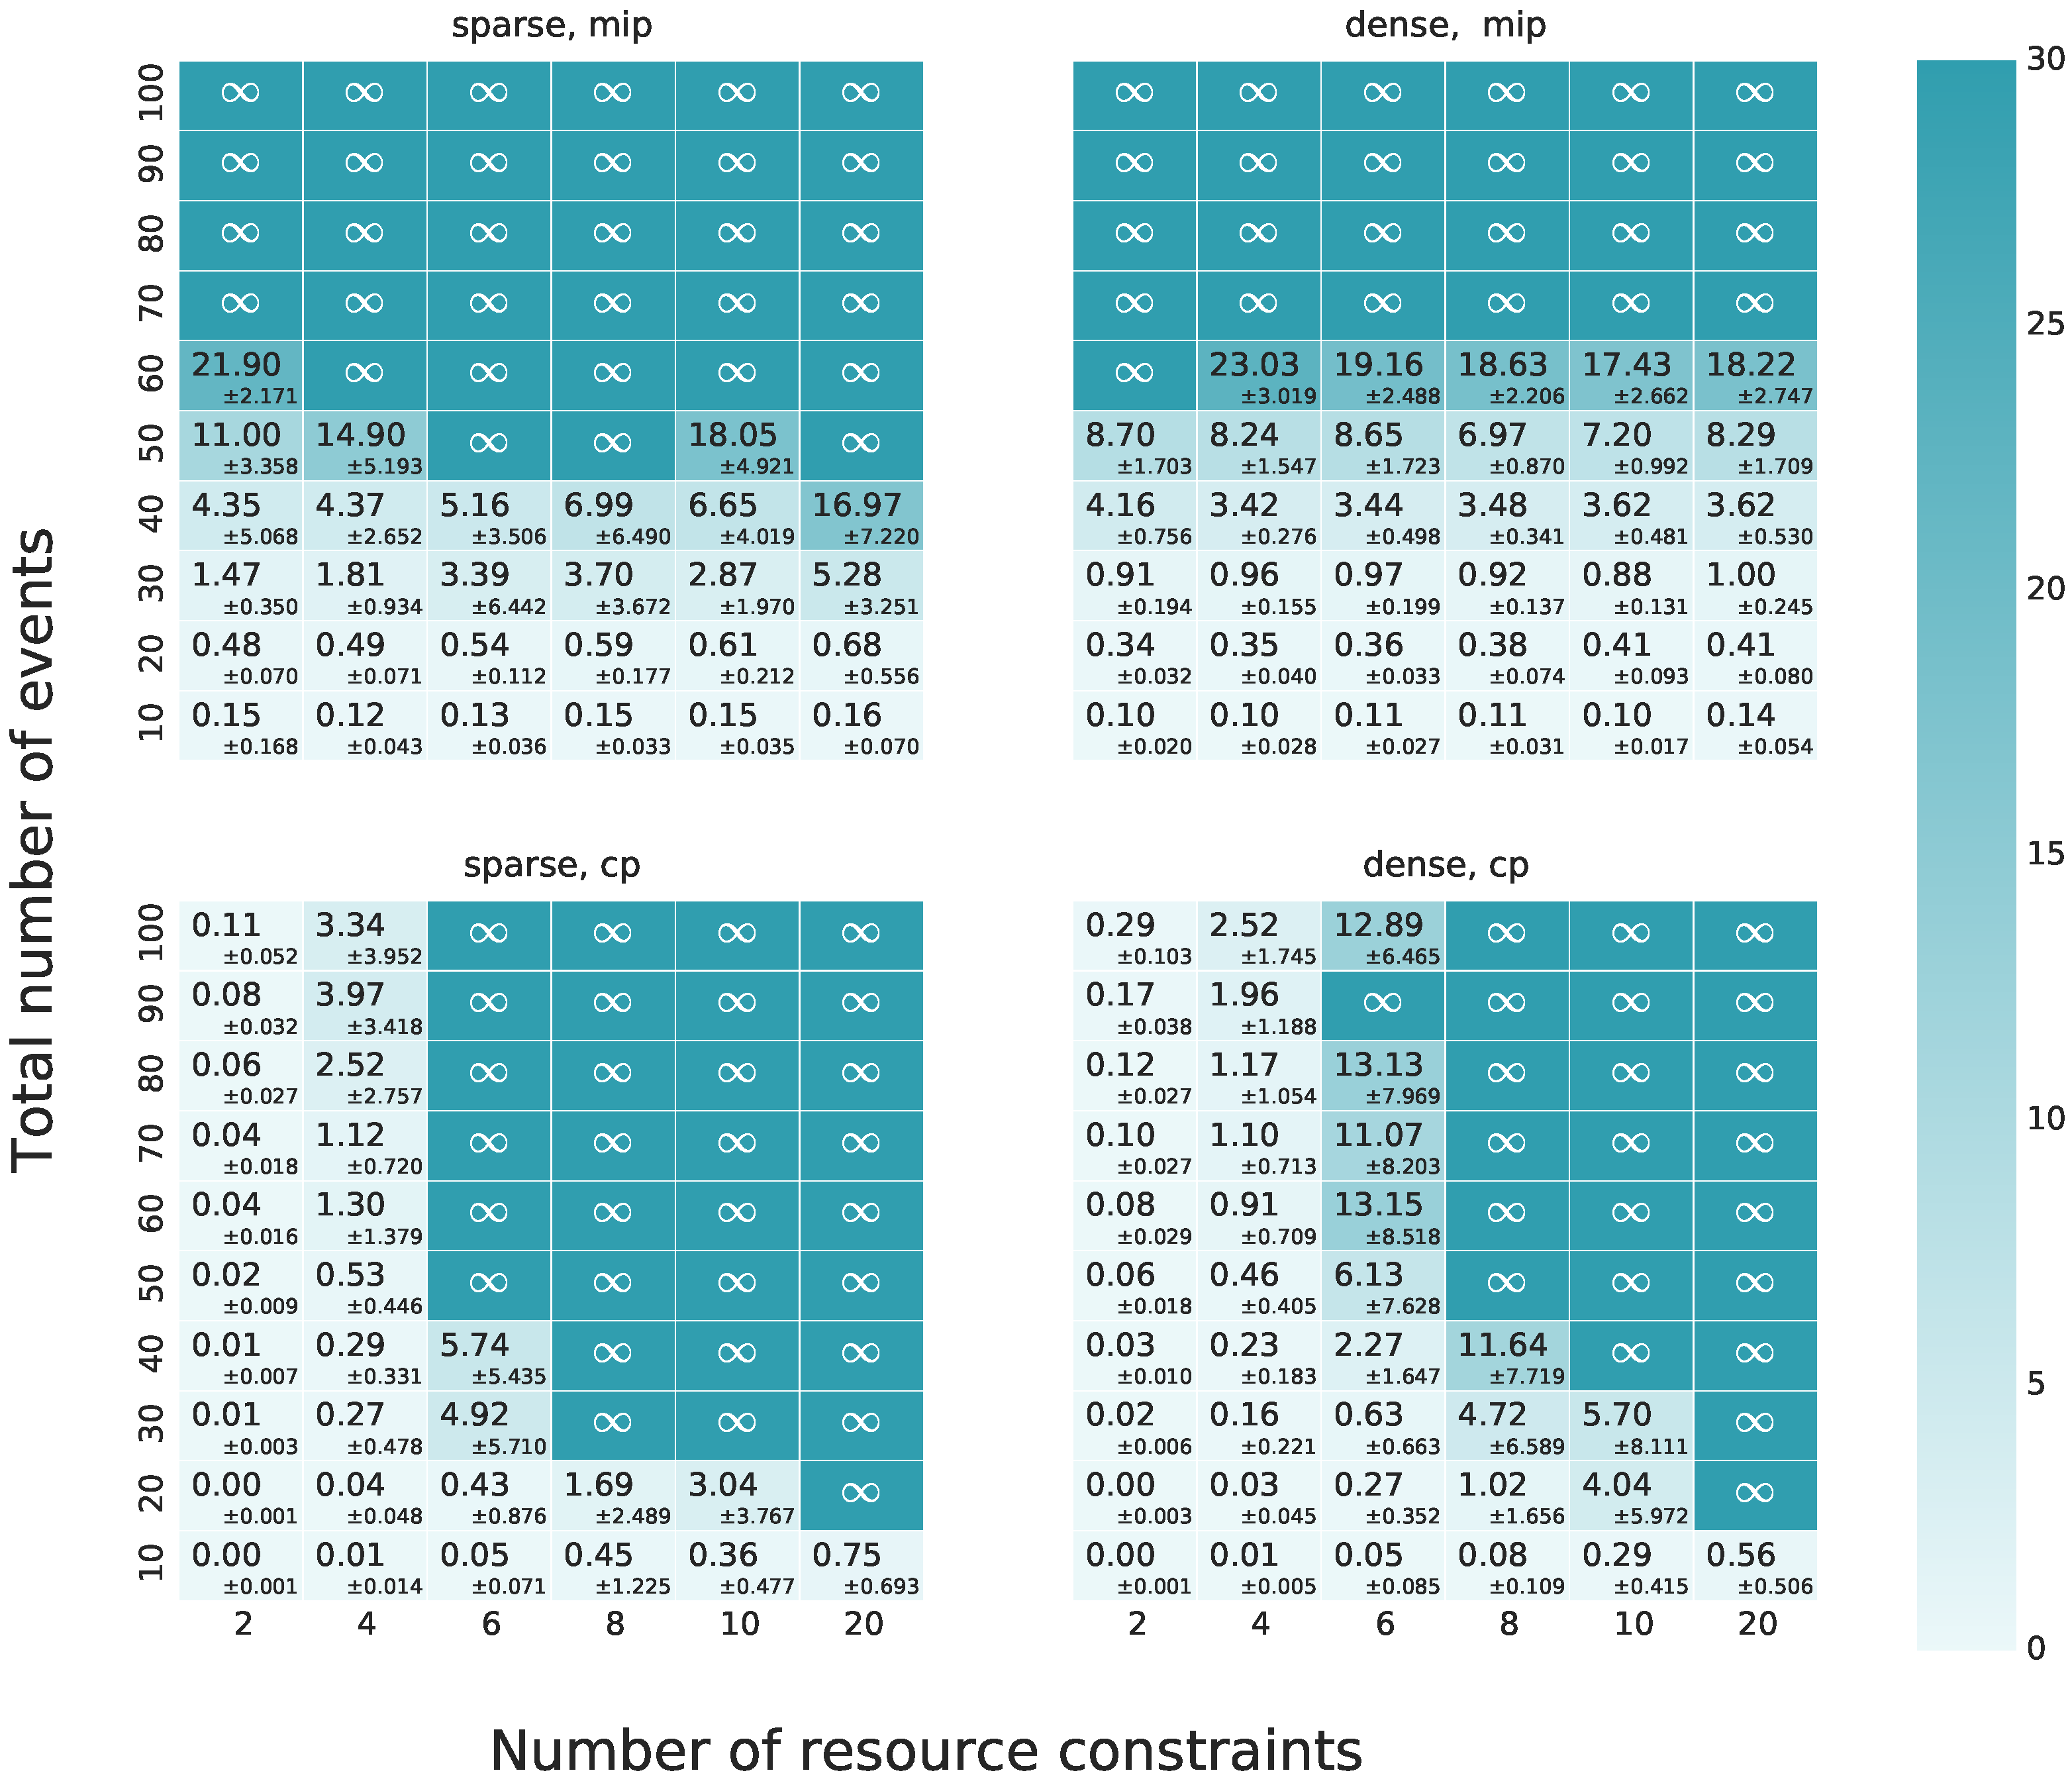
\includegraphics[width=\textwidth]{execution_time_std}
\caption{Comporison of execution time for different types of networks, or $\infty$ if the solver failed to compute the result within the time limit. Y axis represents the number of events in the temporal network ($N$). X axis represents the number of resource constraints ($R$). Top portion of the figure was obtained using the MIP-based solver, while bottom part of the figure was obtained using CP-based solver. The left side of the figure represents computations on \textit{sparse} networks, which in this case means that the total number of temporal constraints is $2N$. On the right side we have \textit{dense} networks, meaning that the number of temporal constraints is $N^2/2$. This figure was computed by running the experiment for every set of parameters multiple times, but each time with different randomly generated instance. Numbers in bottom right corner of each cell are corresponding standard deviations.}
\label{fig:execution_time}
\end{center}
\end{figure*}

\begin{figure*}
\begin{center}
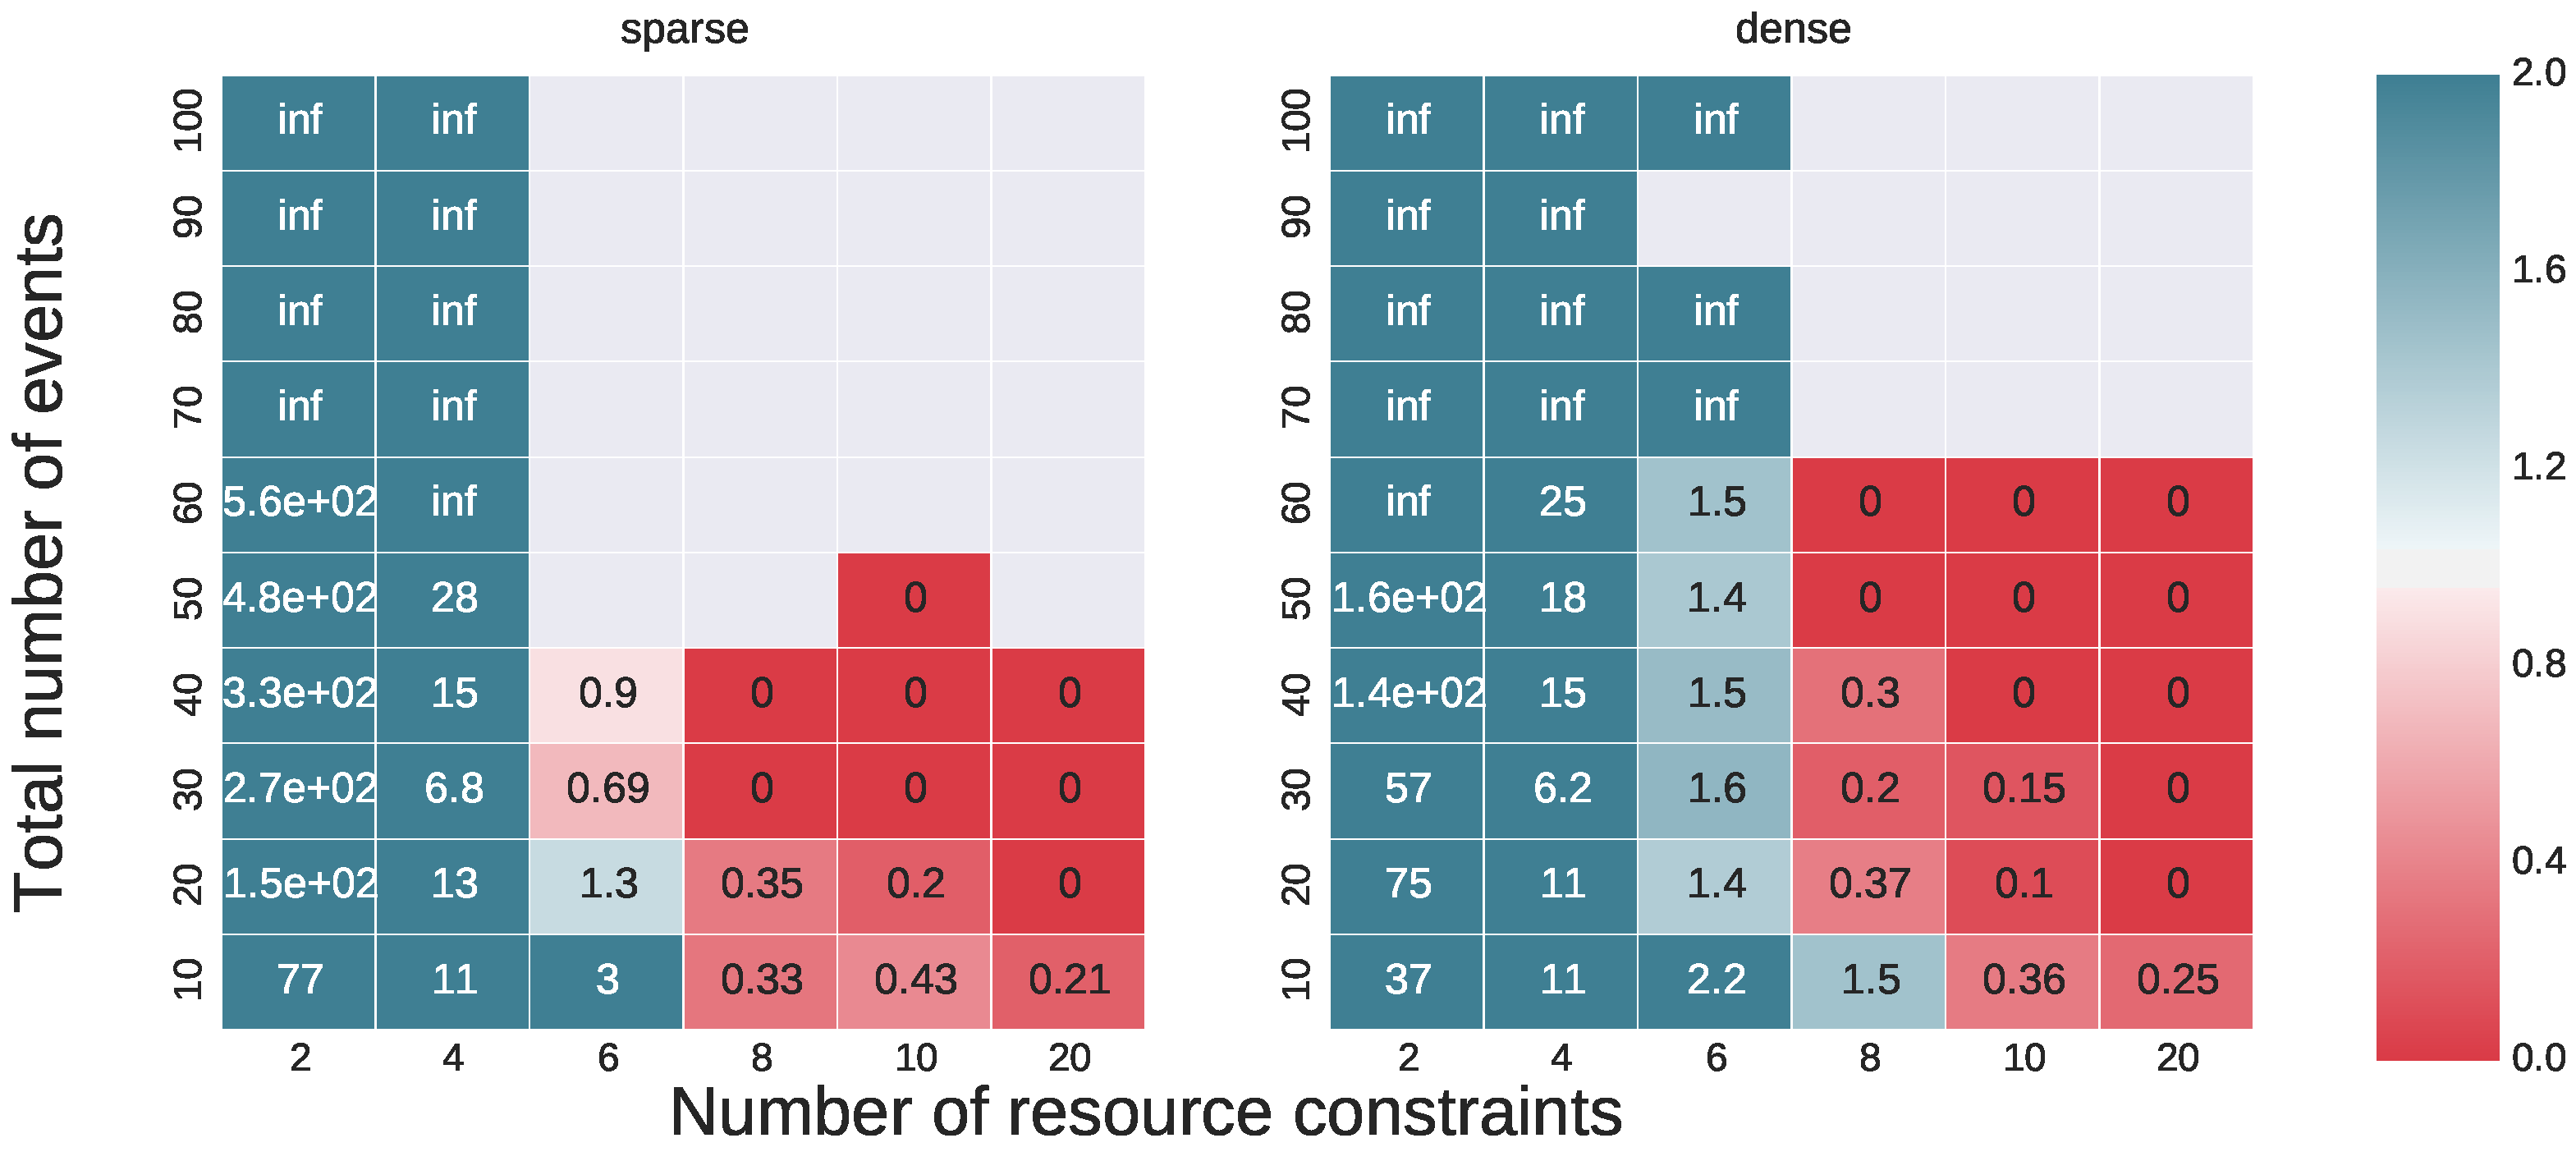
\includegraphics[width=\textwidth]{when_better}
\caption{Number on the figure represents execution time using MIP-based algorithm divided by execution time using CP-based algorithm. Notice that in particular $0$, means that CP-based algorithm failed to compute the results within the time limit and $\infty$ means that MIP-based algorithm timed out. The missing cells correspond to the networks where both of the algorithms timed out and therefore their execution time cannot be compared.   }
\label{fig:when_better}
\end{center}
\end{figure*}

\subsection{TRN over STN}
To understand the performance of our novel CP algorithm, we used the proposed MIP approach as a baseline. We used Gurobi as a MIP solver. Both algorithms were used to determine time-resource consistency for TRN over Simple Temporal Network. In case of MIP based algorithm, all the temporal constraints $l \leq x - y \leq u$, where $l,b \in \mathbb{R}$ and $x,y \in E$ can be expressed as linear constraints, with $x$ and $y$ being continuous variables. In case of CP algorithm, we used Floyd-Warshall to determine temporal consistency as suggested in \cite{dechter1991temporal}. The test cases were created by the following procedure:


% \small{
  \begin{enumerate}
  \setlength\itemsep{0.1em}
  \item Specify number of events $N \geq 2$, number of temporal constraints $T\geq 2$ and number of resource constraints $R\geq 2$
  \item Create a random schedule $s$ for events in $N$ with times in the interval $(0.0, 1.0)$.
  \item Create $T$ time constraints using the following procedure:
    \begin{enumerate}
    \item Choose start and end points $x,y \in N$.
    \item Choose a type of constraint - lower bound or upper bound, each with probability $0.5$
    \item Let $d=s(y) - s(x)$ and chose number $d'$ form exponential distribution with $\lambda = 1 / \sqrt{d}$. For lower-bound set $l = d - d'$. For upper bound set $u = d + d'$.
    \end{enumerate}
  \item Choose number of generating constraints $G$ as a random integer between $1$ and $R-1$ and set number of consuming constraints as $C = R - G$ (so that there's at least on constraint of each type).
  \item Create $G$ generating constraints using the following procedure, by randomly choosing $x,y \in N$ and setting $r$ to a random number between $-1$ and $0$.
  \item Create $C$ consuming constraints using the following procedure.
    \begin{enumerate}
    \item Choose start and end points $x,y \in N$.
    \item Let $m$ be the maximum resource usage value between $x$ and $y$ considering all the resource constraints generated so far. If $m = 0$ repeat the process.
    \item choose $r$ from uniform distribution between $0$ and $-m$.
    \end{enumerate}
  \end{enumerate}
% }

We considered $10$ different values of $N$: $10, 20, ..., 100$. We considered $6$ different values of $R$: $2, 4, 6, 8, 10, 20$. We defined two types of networks - sparse, where $T = 2N$ and dense where $T = N^2/2$. For every set of parameters we run $5$ trials. We set the time limit to $30$ seconds. The results are presented on figure \ref{fig:execution_time}. We can see there exists a set of parameters where only CP managed to find the solution MIP exceed the time limit and vice versa. Figure \ref{fig:when_better} compares execution time of CP and MIP algorithms. The cells colored in blue are the ones where CP algorithm is faster and the cells colored in red are the ones where MIP based algorithm is better. One can see that CP is much better suited for large temporal networks with small number of resource constraints, while MIP scales much better with the number of resource constraints.

\subsection{TRN over pSTN}
To demonstrate extensibility of our approach we have implemented a version of TRN network, where the underlying temporal network is a pSTN (\cite{Fang2014}). pSTN extends the notion of STN. It defines STN-like events and edges as \textbf{actiavated time points} and \textbf{free constraints} respectively. It extends STN with \textbf{received time points}, which are determined by the environment. Every received time point is defined by corresponding \textbf{uncertain duration (uDn)} constraint, which specifies a probability distribution over duration between some activated time point and the received time point. Due to that extension, the notion of consistency $TC(ATN)$ becomes probabilistic; rather than asking \textit{is this pSTN consistent?}, we ask is \textit{is this pSTN consistent with probability $p$?}. Since pSTN is an extension of STN, it is an $ATN$. Given the choice of $p$ we can use probabilistic consistency as $TC$. Therefore we can use CP algorithm to check networks consistency. Example scenario and the schedule obtained by the algorithm is presented in the introduction.
